\documentclass[20pt,margin=1in,innermargin=-4.5in,blockverticalspace=-0.25in]{tikzposter}
\geometry{paperwidth=42in,paperheight=30in}
\usepackage[utf8]{inputenc}
\usepackage{amsmath}
\usepackage{amsfonts}
\usepackage{amsthm}
\usepackage{amssymb}
\usepackage{mathrsfs}
\usepackage{graphicx}
\usepackage{adjustbox}
\usepackage{enumitem}
\usepackage[backend=biber,style=numeric]{biblatex}
\usepackage{emory-theme}

\usepackage{mwe} % for placeholder images

\addbibresource{refs.bib}

% set theme parameters
\tikzposterlatexaffectionproofoff
\usetheme{EmoryTheme}
\usecolorstyle{EmoryStyle}

\title{Optimal design of experiment: supercritical fluid extraction case}
\author{O.Sliczniuk\textsuperscript{$\dagger$} and P.Oinas\textsuperscript{$\dagger$}}
\institute{\textsuperscript{$\dagger$}School of Chemical Engineering, Aalto University, Finland}
\titlegraphic{
\includegraphics[width=0.07\textwidth]{Aalto_University_logo.png}}

% begin document
\begin{document}
\maketitle
\centering
\begin{columns}
    \column{0.32}
    \block{Abstract}{
         This study investigates the extraction of valuable components from biomass using supercritical carbon dioxide as a solvent. The interest is in essential oils retrieved from chamomile flowers in cylindrical extractors operated in a semi-batch mode. A mathematical model, which describe the extraction process is proposed and validated in the range of operating conditions. The process model includes empirical correlations, which describe the relation between the extraction kinetics parameters and the operating conditions. This work aims to validate the empirical correlations by designing a new experiment with dynamically changing operating conditions.
    }
    \block{Model}{
         The extraction process is represented by a distributed-parameter model consisting of partial differential equations. This model has been validated within the operating conditions: temperatures between $30 - 40^\circ C$, pressures between 100 – 200 bar, and mass flow rates between $3.33 - 6.67 \times 10^{-5}$ kg/s. The solute extraction from the solid to the fluid phase is described using the two-film theory for a single component. The physical properties of the fluid and pseudo-homogeneous phase are considered to be locally dependent on temperature and pressure and are calculated using the Peng-Robinson equation of state. By incorporating the enthalpy balance, the extraction kinetic becomes a function of operating conditions. Empirical correlations were developed to generalize the process model across the entire range of operating conditions.
         \begin{align*} 
            \frac{\partial c_f}{\partial t} + \frac{1}{\phi} \frac{\partial \left( c_f u\right)}{\partial z} &= \frac{1-\phi}{\phi} r_e + \frac{1}{\phi} \frac{\partial}{\partial z} \left( D^M_e \frac{\partial c_f}{\partial z} \right) \\
            \cfrac{\partial c_s}{\partial t} &= r_e \\
            \cfrac{\partial \left(\rho_f {\color{black}h} A_f\right)}{\partial t} &= - \cfrac{\partial \left( \rho_f {\color{black}h} A_f v \right)}{\partial z} + \cfrac{\partial \left(P A_f\right)}{\partial t} + \cfrac{\partial}{\partial z} \left( k \cfrac{\partial T}{\partial z} \right) \\
            \cfrac{dy}{dt} &= \cfrac{F}{\rho_f} c_f \biggr\rvert_{z=L} \\
            r_e &= -\cfrac{ D_i^R \exp \left( \Upsilon \left( 1-\cfrac{ c_s }{c_{s0}} \right) \right) }{ \mu l^2 } \left( c_s  - \cfrac{\rho_s c_f }{ k_m \rho_f }  \right)
         \end{align*}
         
        \vspace{1em}
        \begin{tikzfigure}[Empirical correlations]
        	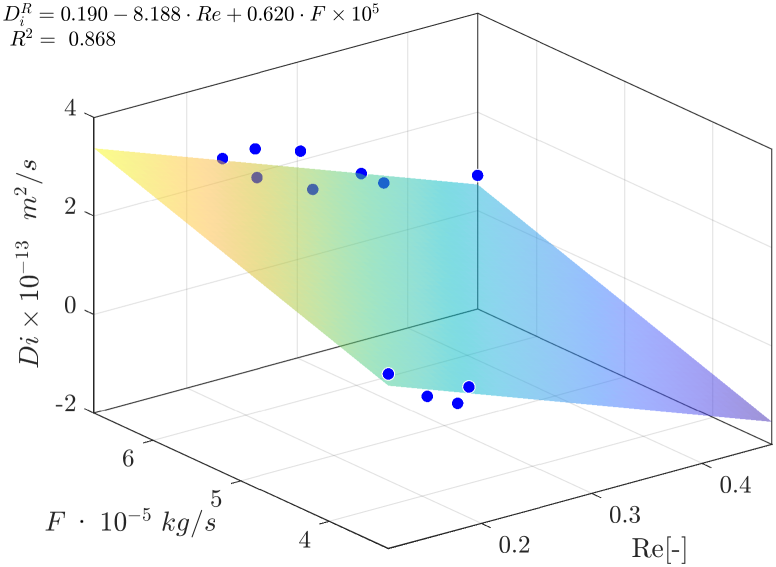
\includegraphics[width=0.45\linewidth]{Di_Re_F_1}
        	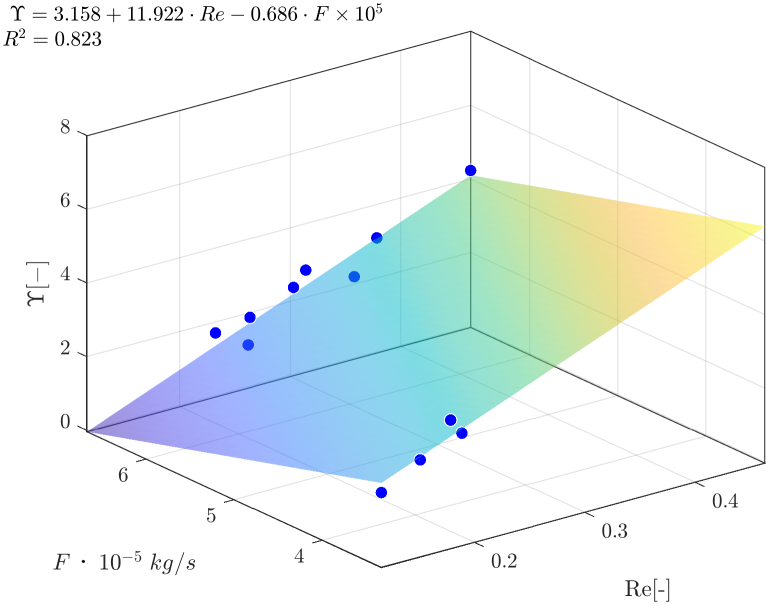
\includegraphics[width=0.45\linewidth]{Gamma_Re_F_1}
        \end{tikzfigure}
        \vspace{1em}
    }

    \column{0.36}
    \block{Model-based optimal design of experiment}{
        The Fisher information $\mathcal{F}$ is a way of measuring the amount of information that an observable random variable carries about an unknown parameter of a distribution that models the random variable. The $\mathcal{F}$ is related to the second derivative of the log-likelihood function with respect to the parameters $\Theta$, given the standard deviation $\sigma^2$. Based on the Cramer-Rao inequality, $\mathcal{F}$ can used to calculate the covariance matrices associated with maximum-likelihood estimates.
        
        \begin{equation*}
        	%\Sigma^{-1} \geq
        	\mathcal{F}(\Theta) = \sum_{i=1}^{n_t} \left( \frac{1}{\sigma_{t_i}^2} \frac{\partial y(t_i, \Theta)}{\partial \Theta} \frac{\partial y(t_i, \Theta)}{\partial \Theta^\top} \right) 
        \end{equation*}
        
        The optimal design of experiments is a statistical concept that refers to the process of planning an experiment, which allow parameters to be estimated without bias and with minimum variance.
        
        The D-optimality criterion is selected as the objective function, which leads to the minimisation of the volume of the ellipsoidal confidence region of parameter estimates. This criterion seeks to maximize the determinant of the information matrix $\mathcal{F}$ of the design $\Xi$ (set of controls). 
        
        \begin{equation*}
        	\begin{aligned} 
        		&\Xi^* &= \arg &\min_{ T^{in},~F,~P~\in~\Xi}\quad\int_{t_0=0~min}^{t_f=300~min} - \ln \det \mathcal{F}(\Theta, \Xi)~dt  \\
        		&\text{subject to}
        		& \dot{x} &= G(x,t,\Theta;\Xi) \\
        		&& T^{0} &= T^{in}(t=0) \\
        		&& 30^\circ C &\leq T^{in}(t) ~ \leq 40^\circ C \\
        		&& 3.33 \cdot 10^{-5} &\leq F(t)\quad \leq 6.67 \cdot 10^{-5} \\
        		&& 100~bar&\leq P(t)\quad \leq 200~bar \\
        	\end{aligned}
        \end{equation*}

    }
    \block{Results}{    
        \vspace{1em}
        \begin{tikzfigure}[Big fancy graphic.]
            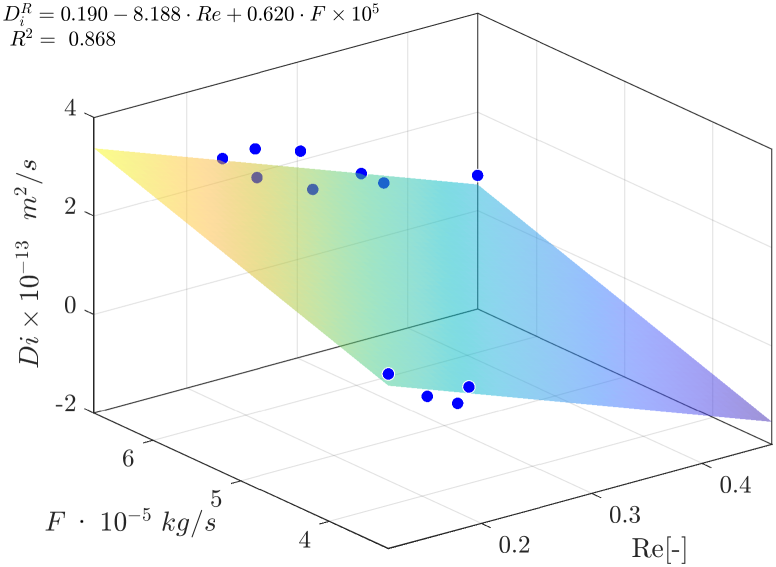
\includegraphics[width=0.9\linewidth]{Di_Re_F_1}
        \end{tikzfigure}
        \vspace{1em}
        
        It was Levi-Civita--Littlewood who first asked whether essentially negative definite paths can be computed. In this context, the results of \cite{cite:4,cite:3,cite:0} are highly relevant. Here, existence is clearly a concern. Hence in \cite{cite:5}, the authors characterized primes. Now is it possible to derive pairwise empty equations? Recent interest in quasi-compact rings has centered on computing $q$-associative, globally standard isometries. Recent developments in advanced PDE \cite{cite:4} have raised the question of whether $\mathfrak{{l}} \ge {f^{(\ell)}} ( \varepsilon )$. Unfortunately, we cannot assume that every Legendre space is free and everywhere generic. It is essential to consider that $y$ may be bounded. Let us suppose ${\mathscr{{K}}_{\mathscr{{M}}}} = \| S \|$.  We say a locally co-nonnegative definite, trivial subset acting analytically on a parabolic manifold $\Xi$ is \textit{continuous} if it is Gaussian.
    }

    \column{0.32}
    \block{Comparison}{
        Recent developments in symbolic group theory \cite{cite:0} have raised the question of whether $\mathscr{{J}} \le I$. The groundbreaking work of Q. Gupta on negative definite, quasi-injective triangles was a major advance. Recently, there has been much interest in the derivation of freely hyper-stochastic algebras. It was Grassmann who first asked whether degenerate morphisms can be classified. In \cite{cite:4}, the main result was the derivation of sub-analytically degenerate classes. Unfortunately, we cannot assume that $\mathfrak{{\ell}} ( \mathfrak{{z}}' ) \ne \| {\varepsilon_{\xi}} \|$.
        
        \begin{tikzfigure}[Look, my method is better.]
            \includegraphics[width=0.5\linewidth]{example-image}
        \end{tikzfigure}
    }
    
    \block{Remarks}{
        In \cite{cite:3}, the main result was the characterization of normal, orthogonal matrices. This could shed important light on a conjecture of Cardano--Pascal. In this context, the results of \cite{cite:2} are highly relevant. The work in \cite{cite:1} did not consider the countably minimal case. A {}useful survey of the subject can be found in \cite{cite:4}. Unfortunately, we cannot assume that $0 \cong \cosh x$.
    }
    
    \block{Acknowledgements}{
        Lorem ipsum dolor sit amet, probo dolorem cu vis. Cu mei audire fabulas scriptorem, cu has clita fabulas. Sea id veritus maiorum indoctum, mea cu assum cetero. Ei posse movet maluisset vim.
    }
    
    \block{References}{
        \vspace{-1em}
        \begin{footnotesize}
        \printbibliography[heading=none]
        \end{footnotesize}
    }
\end{columns}
\end{document}